	\documentclass[../pfc.tex]{subfiles}

	\begin{document}
	
	\section{Parte App móvil}
	
	\section{Arquitectura}
	
	Como se ha comentado antes en este documento Scrum y las tecnologías ágiles, por su forma de enfocar las tareas y el propio desarrollo en un equipo con un nivel técnico que no sea excelente, si no se introducen medidas paliativas que corrijan esto, suelen obtener diseños arquitecturales de clases un poco pobres, tendentes al acoplamiento y poco cohesionado. Para paliar esto se suelen introducir historias de usuario de reducción de deuda técnica, o de refactorización de todo el código existente, así como herramientas que detecten code smells\cite{refactoring} o malas practicas de desarrollo.\\ 
	
	Estas herramientas pueden incluir plugins del IDE que hagan análisis estático de código y pueden advertirnos sobre puntuales problemas dentro de una clase, pero poco hay a nivel de las relaciones entre las mismas, fuera del uso de patrones de diseño conocidos, y aun en las relaciones entre estos patrones que son bloques más grandes de código. Es por eso que creemos que hay que establecer unas líneas base al principio del proyecto sobre la arquitectura de la propia aplicación. En principio serán ciertamente vaguedades y lugares comunes sobre el desarrollo en capas, aislamiento de las mismas etc, pero si a través de los sprints reservamos un poco de tiempo en la reunión de sprint planning para conversar sobre las historias del propio sprint, en que capa encajan, como deberían hablar las capas entre sí si son mas de una las involucradas en la historia, etc ademas de con las historias de deuda técnica si fuesen necesarias creemos que puede solventarse en gran medida esa falta de bueno diseño y arquitectura que se achaca a las metodologías ágiles.\\
	
	
		\begin{figure}[H]
			\centering
			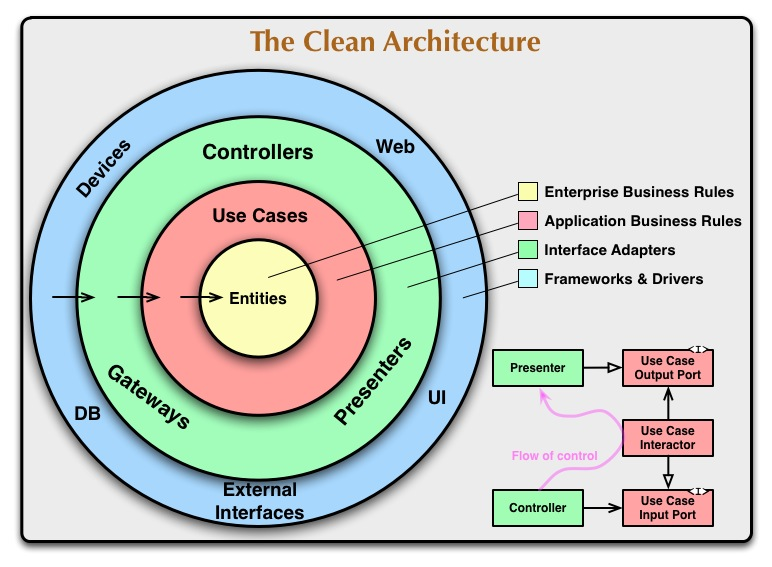
\includegraphics[width=0.8\linewidth]{../images/CleanArchitecture}
			\caption{Arquitectura 'limpia' propuesta por Robert Martin}
			\label{fig:cleanarch}
		\end{figure}
	
	Para hablar de arquitectura hemos tomado como referencia Clean Architecture\cite{cleanarch} propuesta por Robert C. Martin aunque es muy similar a la Arquitectura Cebolla de Jeffrey Palermo\cite{onion} o la Arquitectura Hexagonal de Alaister Cockburn\cite{onion}. Todas ellas se basan por hacer capas fuertemente cohesionadas dentro de cada una pero con nulo conocimiento fuera de las mismas que se comunican mediante interfaces públicos ofrecidos al resto de capas. Esto y la propagación hacia el interior, esto es que cada capa solo hablara con la que tiene arquitecturalmente en un nivel superior o inferior. Esto es la capa de UI que es la que interactuá con el usuario solamente invocará métodos de la interfaz de la capa de vista que es la que conceptualmente tiene justo encima. Esta solamente interactuará con la capa de UI antes mencionada y con la capa del presentador, y así sucesivamente. \\
	
	\subsection{Ley de Deméter}
	
	La idea subyacente bajo todas estas arquitecturas de capas que no se conocen, es la Ley de Deméter. Que en su enunciado mas simple dice:
		\begin{itemize} 
			\item Cada unidad debe tener un limitado conocimiento sobre otras unidades y solo conocer aquellas unidades estrechamente relacionadas a la unidad actual.
			\item Cada unidad debe hablar solo a sus amigos y no hablar con extraños.
			\item Solo hablar con sus amigos inmediatos.
		\end{itemize}
	La noción fundamental es que dado un objeto, este debería asumir tan poco como sea posible sobre la estructura o propiedades de cualquier otro (incluyendo sus subcomponentes).\\
	
	Aplicando la ley a la orientación a objetos a la Ley de Deméter puede ser llamada más precisamente la "Ley de Deméter para funciones/Métodos" (LD-F). En este caso, un objeto A puede solicitar un servicio (llamar a un método) de un objeto B, pero el objeto A no debería "llegar a través" del objeto B poder acceder a otro objeto, C, para solicitar sus servicios. De hacerlo podría significar que el objeto A implícitamente requeriría un mayor conocimiento de la estructura interna del objeto B. En su lugar, la interfaz de B debe ser modificado si es necesario para que pueda servir directamente la petición de A, propagándolo a cualquiera de sus subcomponentes necesarios. Alternativamente, A podría tener una referencia directa al objeto C y hacer la solicitud directamente a él. Si la ley se sigue, B es el único objeto que debería conocer su propia estructura interna.\\
	
	Más formalmente, la Ley de Deméter para funciones requiere que un método m de un objeto O sólo se puede invocar los métodos de los siguientes tipos de objetos:
	\begin{itemize} 
		\item El propio O
		\item Los parámetros de m
		\item Cualquier objeto creado / instanciados dentro de m
		\item Objetos que sean propiedades de O
		\item Una variable global, accesible por O, en el ámbito de m
	\end{itemize}
	
	En particular, un objeto debe evitar invocar métodos de un objeto miembro devuelto por otro método. Para muchos lenguajes orientados a objetos modernos que usan un punto como identificador de campo, la ley puede se puede resumir simplemente como "usar sólo un punto". Es decir, el a.b.Method() rompe la ley mientras que a.Method() no lo hace. Como analogía, cuando uno quiere que un perro ande, no se ordena a las patas del perro a caminar directamente, sino que se manda al perro que luego manda sus propias piernas.\\
		
	Con esto en mente en mente construiremos tres grandes capas que serán las típicas de vista, dominio y datos. Cada capa despues tendrá sus propios patrones o entidades de patrones, y alguna subcapa. Lo importante es que cada capa ofrezca un interfaz a las capas que tienen que interactuar con ella y que estas solamente conocerán dicho interfaz.  \\
	
	Como frontera entre la vista y el dominio pondremos un patrón de MVP o Modelo-Vista-Presentador, este patrón es una modificación del Modelo-Vista-Controlador que sirve para separar de la vista y representación gráfica de nuestros objetos de modelo, de la representación de estos. En este modelo la vista es lo más "tonta" o simple posible de manera que no merezca la pena testarse. Y los eventos sobre la misma se los comunicará al presentador que será el encargado de lidiar con el modelo de los objetos de negocio de la aplicación.  
	
	\subsection{Capa de Vista}
	
	Esta capa contendrá toda la parte de UI, que será lo más tonta posible. Esto es, contendrá los elementos de UI para pintar y actualizar la pantalla del dispositivo, pero cualquier acción realizada por el usuario en una pantalla, será notificada al presenter que será el que siguiendo el caso de uso tome la decisión adecuada.\\ 
	
	
	\subsection{Capa de Dominio}
	
	Esta capa implementará los casos de uso de la app así como las entidades del dominio de la misma. De este modo contendrá los presentadores de los casos de uso y los casos de uso mismos del diagrama anterior que se comunicaran mediante una interfaz. Los presentadores se comunicarán también, vía interfaz, con las vistas tontas de la capa de UI.\\
	
	
	\subsection{Capa de Datos}
	
	Esta será la capa de acceso a los datos donde residan las llamadas a servicios web para la obtención o persistencia de los mismos, así como las clases que nos ayuden a interactuar con la base de datos del dispositivo. En esta capa aplicaremos un patrón repositorio sobre las entidades de la capa. Esto hará que independicemos el medio de obtención de los datos que podrá ser una base datos, una cache, un servicio web, etc.
	Aparte de la capa de modelo nos llegarán operaciones con los datos y será esta capa quien decida si debe actualizar los mismos en base de datos o no y si además debe hacer backup de los mismos para poder mantener los dispositivos sincronizados.\\
	
	
	\subsection{Principios SOLID}
	
	Todo esto se ha de implementar siguiendo los principios de SOLID\cite{solid} que nos muestran en cinco pequeños principios de escritura de software como escribir código reusable, con alta cohesión y bajo acoplamiento, que es por otra parte lo que deseábamos lograr al principio de la sección.
	
	
	\subsubsection{S-Responsabilidad única (Single responsibility)}
	
	Este principio dice que cada clase debe ocuparse de un solo menester sencillo y concreto. Visto de otro modo, dice que cada clase debería tener un único motivo para ser modificada. En muchas ocasiones estamos tentados a poner un método reutilizable que no tienen nada que ver con la clase simplemente porque lo utiliza y pilla más a mano. \\
	
	El problema surge cuando tenemos la necesidad de utilizar ese mismo método desde otra clase. Si no se refactoriza en ese momento y se crea una clase destinada para la finalidad del método, nos toparemos a largo plazo con que las clases realizan tareas que no deberían ser de su responsabilidad.\\
	
	Con la anterior mentalidad nos encontraremos, por ejemplo, con un algoritmo de formateo de números en una clase destinada a leer de la base de datos porque fue el primer sitio donde se empezó a utilizar. Con otro ejemplo si estamos delante de una clase que se podría ver obligada a cambiar ante una modificación en la base de datos y a la vez, ante un cambio en el proceso de negocio, podemos afirmar que dicha clase tiene más de una responsabilidad o más de un motivo para cambiar. Esto conlleva a tener métodos difíciles de detectar y encontrar de manera que el código hay que tenerlo memorizado en la cabeza.\\
	
	Se aplica tanto a la clase como a cada uno de sus métodos, con lo que cada método también debería tener un solo motivo para cambiar. El efecto que produce este principio son clases con nombres muy descriptivos y por tanto largos, que tienen menos de cinco métodos, cada uno también con nombres que sirven perfectamente de documentación, es decir, de varias palabras: CalcularAreaRectangulo y que no contienen más de 15 líneas de código.\\
	
	
	\subsubsection{O-Abierto/Cerrado (Open/Closed)}
	
	Principio que habla de crear clases extensibles sin necesidad de entrar al código fuente a modificarlo. Generalizando una entidad software (una clase, módulo o función) debe estar abierta a extensiones pero cerrada a modificaciones. Es decir, el diseño debe ser abierto para poderse extender pero cerrado para poderse modificar. Aunque dicho parece fácil, lo complicado es predecir por como se debe extender y que no tengamos que modificarlo. Para conseguir este principio hay que tener muy claro como va a funcionar la aplicación, por donde se puede extender y como van a interactuar las clases.\\
	
	El uso más común de extensión es mediante la herencia y la reimplementación de métodos de la clase padre que podría incluso ser abstracta. La otra podría ser inyectando dependencias que cumplen el mismo contrato (que tienen la misma interfaz) pero que implementan diferente funcionamiento. En todos los casos, el comportamiento de la clase cambia sin que hayamos tenido que modificar código interno.\\
		
	Como la totalidad del código no se puede ni se debe cerrar a cambios, el diseñador debe decidir contra cuáles protegerse mediante este principio. Su aplicación requiere bastante experiencia, no sólo por la dificultad de crear entidades de comportamiento extensible sino por el peligro que conlleva cerrar determinadas entidades o parte de ellas.\\
	
	Como ya he comentado llega un momento en que las necesidades pueden llegar a ser tan imprevisibles que nos topemos que con los métodos definidos en el interface o en los métodos extensibles, no sean suficientes para cubrir las necesidades. En este caso no habrá más remedio que romper este principio y refactorizar.\\
	
	Cerrar en exceso obliga a rescribir demasiadas líneas de código a la hora de reutilizar la entidad en cuestión. \\
	
	
	\subsubsection{L-Sustitucion Liskov (Liskov substitution)}
	
	Este principio habla de la importancia de crear todas las clases derivadas para que también puedan ser tratadas como la propia clase base. Cuando creamos clases derivadas debemos asegurarnos de no reimplementar métodos que hagan que los métodos de la clase base no funcionases si se tratasen como un objeto de esa clase base.\\
	
	Algo más formal, lo que viene diciendo es que si una función recibe un objeto como parámetro, de tipo X y en su lugar le pasamos otro de tipo Y, que hereda de X, dicha función debe proceder correctamente.\\
	
	Por el propio polimorfismo, los compiladores e intérpretes admiten este paso de parámetros, la cuestión es si la función de verdad está diseñada para hacer lo que debe, aunque quien recibe como parámetro no es exactamente X, sino Y.\\
	
	El principio de sustitución de Liskov está estrechamente relacionado con el anterior en cuanto a la extensibilidad de las clases cuando ésta se realiza mediante herencia o subtipos. Si una función no cumple el LSP entonces rompe el OCP puesto que para ser capaz de funcionar con subtipos (clases hijas) necesita saber demasiado de la clase padre y por tanto, modificarla. El diseño por contrato (Design by Contract) es otra forma de llamar al LSP.\\
	
	
	\subsubsection{I-Segregacion del interface (Interface segregation)}
	
	Este principio trata de algo parecido al primer principio. Cuando se definen interfaces estos deben ser específicos a una finalidad concreta es por ello que defiende que no obliguemos a los clientes a depender de clases o interfaces que no necesitan usar. Por ello, si tenemos que definir una serie de métodos abstractos que debe utilizar una clase a través de interfaces, es preferible tener muchos interfaces que definan pocos métodos que tener un interface con muchos métodos. Ya que de lo contrario seguramente sirve a varios objetos cliente con responsabilidades diferentes, con lo que debería estar dividida en varias entidades.\\
	
	El objetivo de este principio es principalmente poder reaprovechar los interfaces en otras clases. Si tenemos un interface que compara y clona en el mismo interface, de manera más complicada se podrá utilizar en una clase que solo debe comparar o en otra que solo debe clonar.\\
	
	En los lenguajes como Java y C\# hablamos de interfaces pero en lenguajes interpretados como Python, que no requieren interfaces, hablamos de clases. No sólo es por motivos de robustez del software, sino también por motivos de despliegue. Cuando un cliente depende de una interfaz con funcionalidad que no utiliza, se convierte en dependiente de otro cliente y la posibilidad de catástrofe frente a cambios en la interfaz o clase base se multiplica.\\
	
	
	\subsubsection{D-Inversión de dependencias (Dependency inversion)}
	
	El objetivo de este principio conseguir desacoplar las clases. En todo diseño siempre debe existir un acoplamiento pero hay que evitarlo en la medida de lo posible. Un sistema no acoplado no hace nada pero un sistema altamente acoplado es muy difícil de mantener. La inversión de dependencias da origen a la conocida inyección de dependencias, una de las mejores técnicas para lidiar con las colaboraciones entre clases, produciendo un código reutilizable, sobrio y preparado para cambiar sin producir efectos bola de nieve.\\
	
	El objetivo de este principio es el uso de abstracciones para conseguir que una clase interactúe con otras clases sin que las conozca directamente. Es decir, las clases de nivel superior no deben conocer las clases de nivel inferior. Dicho de otro modo, no debe conocer los detalles. Existen diferentes patrones como la ya mencionada inyección de dependencias o service locator que nos permiten invertir el control.\\
		
	DIP explica que un módulo concreto A, no debe depender directamente de otro módulo concreto B, sino de una abstracción de B. Tal abstracción es una interfaz o una clase (que podría ser abstracta) que sirve de base para un conjunto de clases hijas.\\
	
	En el caso de un lenguaje interpretado no necesitamos definir interfaces, ni siquiera jerarquías pero el concepto se aplica igualmente. Veámoslo con un ejemplo sencillo: La clase \textbf{Logica} necesita de un colaborador para guardar el dato \textbf{Dato} en algún lugar persistente. Disponemos de una clase \textbf{MyBD} que es capaz de almacenar \textbf{Dato} en una base de datos MySQL y de una clase \textbf{FS} que es capaz de almacenar \textbf{Dato} en un fichero binario sobre un sistema de ficheros NTFS.\\
	
	Si en el código de \textbf{Logica} escribimos literalmente el nombre de la clase \textbf{MyBD} como colaborador para persistir datos, ¿Cómo haremos cuando necesitamos cambiar la base de datos por ficheros binarios en disco?. No quedará otro remedio que modificar el código de \textbf{Logica}.\\
	
	Si las clases \textbf{MyDB} y \textbf{FS} implementasen una misma interfaz \textbf{IPersistor} para guardar \textbf{Dato}, podríamos limitarnos a usar \textbf{IPersistor} (que es una abstracción) en el código de \textbf{Logica}. Cuando los requerimientos exigiesen un cambio de base de datos por ficheros en disco o viceversa, sólo tendríamos que preocuparnos de que el atributo \textbf{\_myPersistor} de la clase \textbf{Logica}, que es de tipo \textbf{IPersistor} contuviese una instancia de \textbf{MyDB} o bien de \textbf{FS}.\\
	
	¿Cómo resolvemos esta última parte?. Con la inyección de dependencias, que es una técnica que como ya hemos dicho se usa para obtener la Inversión de Dependencias.\\
	
	Como se ha comentado la arquitectura de la aplicación divide a esta entres capas que saben lo minimo unas de otras y que se comunican por interfaces, a modo de contrato para ocultar tras esto la implementación de las clases que cumpliran dicho contrato.
	
	\section{Diagrama de Clases}
	
		Como se ha comentado la arquitectura de la aplicación divide a esta entres capas que saben lo minimo unas de otras y que se comunican por interfaces, a modo de contrato para ocultar tras esto la implementación de las clases que cumpliran dicho contrato.
		
	
	\subsection{Capa de Datos}
	
	La capa de datos se comunica con el dominio implementando las clases Repository de cada entidad, que marcan las operaciones a realizar con las mismas. Tras implementar dicho interfaz, aplica un a su vez un patrón repository para definir las operaciones con las entidades y auxiliares. Mediante una factoria de DataStores decidiremos la estrategia para acceder o guardar las entidades, por ejemplo podriamos establecer una implementación mediante caché, si el elemento esta en caché la factoria devolverá un CacheDataStore y si por contra no se encuentra en caché, devolvera un DatabaseDataStore para traerlo de la base de datos, actualizando la caché. Esta capa maneja las entidades Entity que transforma en entidades de dominio cuando le solicitan operaciones. 
		
		\begin{figure}[H]
			\centering
			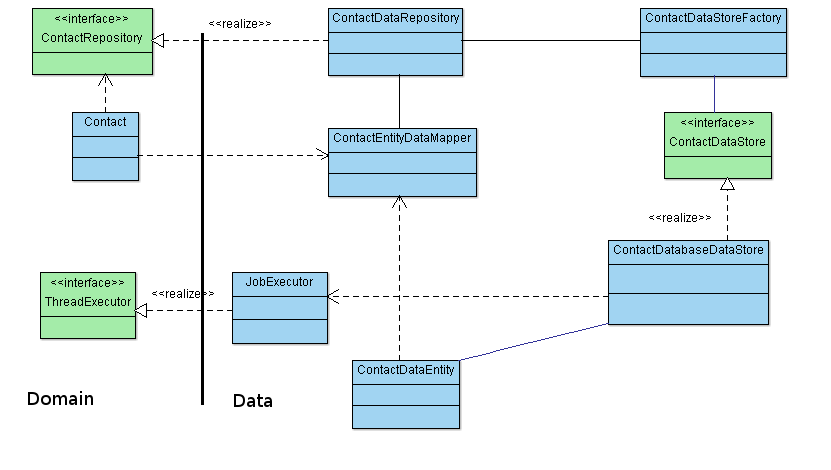
\includegraphics[width=0.8\linewidth]{../images/DataClasesDiagram}
			\caption{Diagrama de clases de la capa de datos}
			\label{fig:Clases de la capa Data}
		\end{figure}
		
	\subsection{Capa de Dominio}
	
	La capa de dominio esta basada en los casos de uso de la aplicación. Estos son interfaces que heredan de Interactor, que implementa Runable. De esta manera las implementaciones de los mismos contienen un ThreadExecutor implementado por JobExecutor en la capa de datos, al que se envian a si mismos para ejecutar la acción del caso de uso. Por el otro lado, son los diferentes presenters de la aplicación, quienes implementan los diferentes casos de uso. 
		
			\begin{figure}[H]
				\centering
				\includegraphics[width=0.8\linewidth]{../images/DomainClasesDiagram}
				\caption{Diagrama de clases de la capa de dominio}
				\label{fig:Clases de la capa Domain}
			\end{figure}
		
	\subsection{Capa de Presentación}
	
	Esta capa se relaciona con el dominio mediante los presenters, que contienen las operaciones de los diferentes casos de uso que se relacionan en su vista. Ademas contienen interfaces sobre las clases de vista para que estas soporten los metodos que los propios presenters necesitan.
	
			\begin{figure}[H]
				\centering
				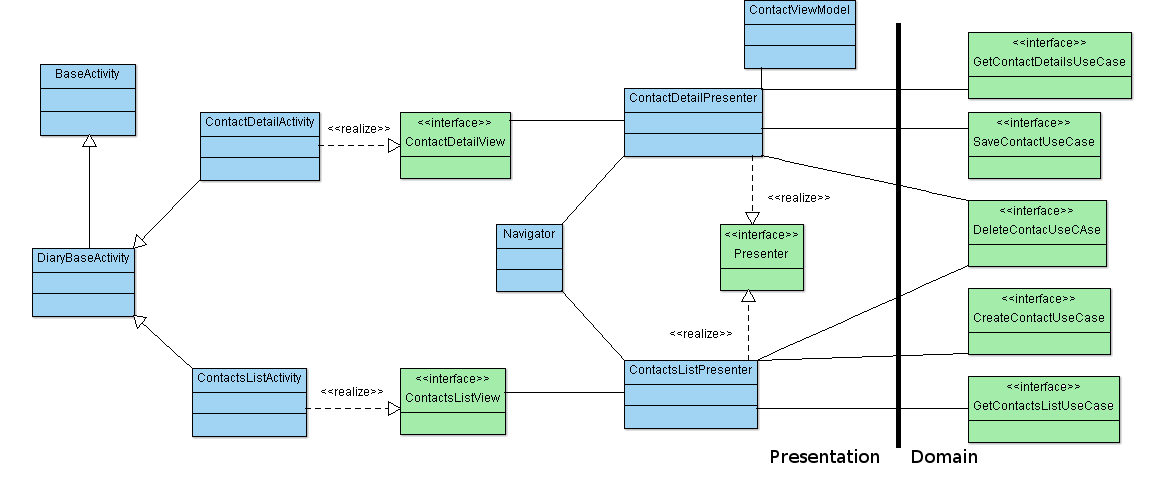
\includegraphics[width=0.8\linewidth]{../images/PresentationClasesDiagram}
				\caption{Diagrama de clases de la capa de presentación}
				\label{fig:Clases de la capa Presentation}
			\end{figure}
	
	\section{Diagrama de Clases}
	


	\section{Diagrama E/R de la base de datos}
	

	Para el diseño de la base de datos incluida dentro de la aplicación y que va a utilizarse para tratar la información introducida por el usuario, hemos recreado un diagrama sencillo de tipo Entidad-Relación en el que se muestran las entidades que serán llevadas a tablas y sobre las que se realizarán las típicas operaciones de creación, lectura, actualización y borrado (CRUD).

	
		\subsection{Diagrama}
		
		\begin{figure}[H]
			\centering
			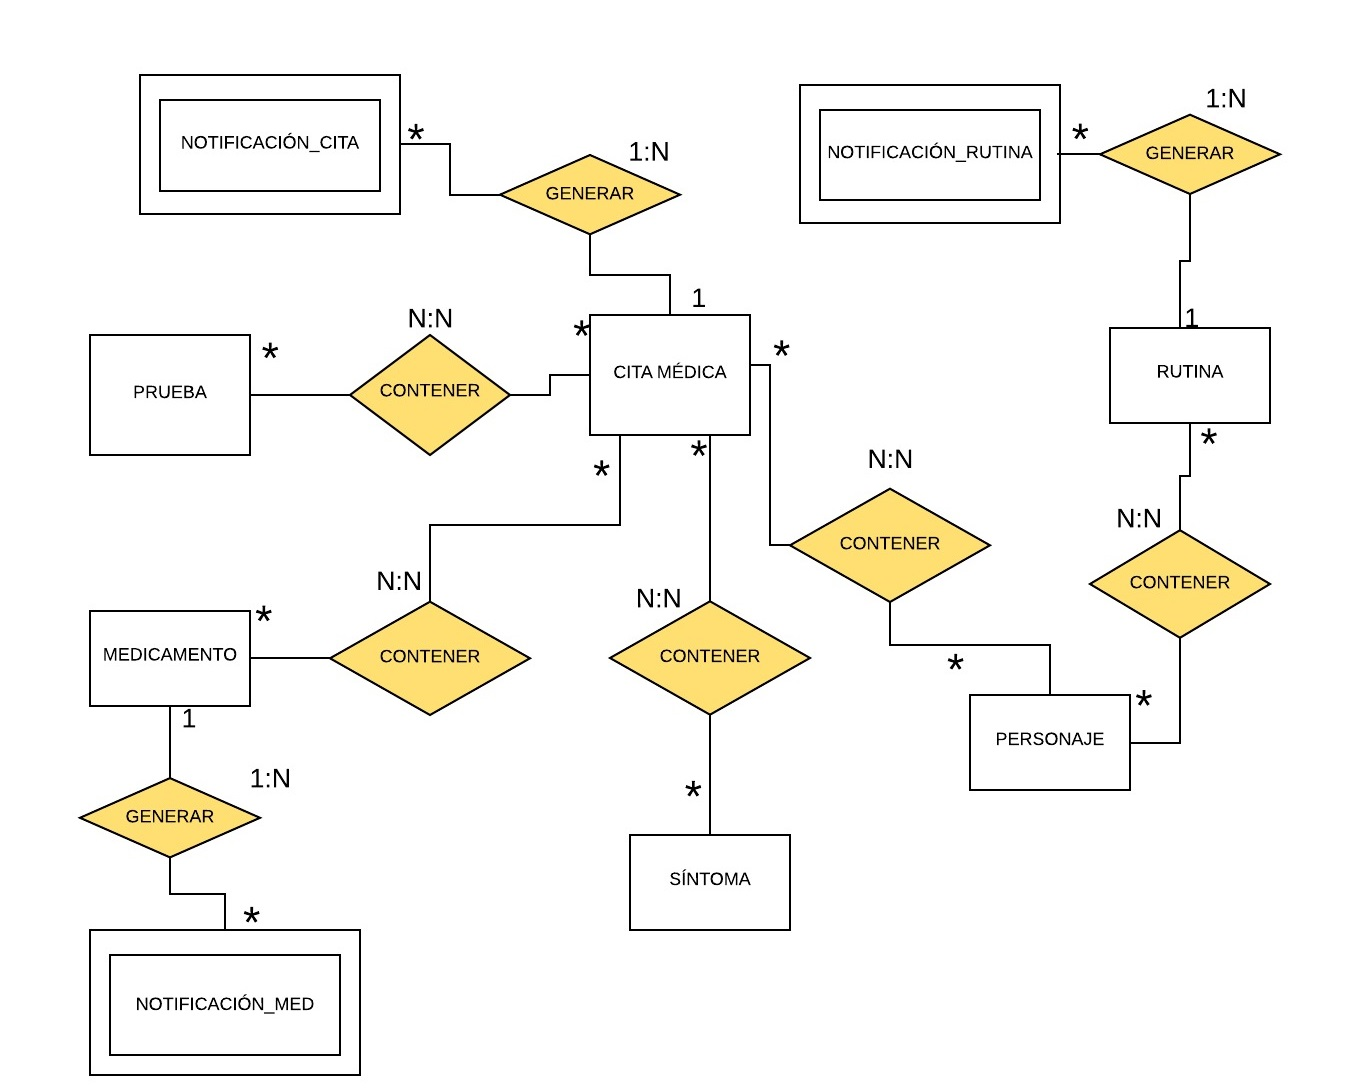
\includegraphics[width=1\linewidth]{../images/diagrama_e_r}
			\caption{Diagrama entidad relación de la base de datos local}
			\label{fig:diagramaer}
		\end{figure}
		
		\subsection{Descripción}
		
		El diagrama de la figura anterior\cite{diagramaer} es el diseño en papel de la base de datos local, la que tendrá el usuario en su móvil en la aplicación.
		
		Consta de varias entidades fuertes o formales:
		
		\begin{itemize}
			\item Cita médica; Sus atributos son id (PK), nombre, lugar, descripción, día de cita, hora de cita, día a notificar , hora a notificar, duración e imagen.
			
			\item Rutina; Sus atributos son id (PK), nombre, lugar, descripción, día de rutina, hora de rutina, día a notificar, hora a notificar, duración, satisfacción e imagen.
			
			\item Personaje; Sus atributos son id (PK), nombre, apellidos, dirección,  teléfono, relación, imagen.
			
			\item Medicamento; Sus atributos son id (PK), nombre, descripción, día inicio, hora inicio, día fin, hora fin, intervalo, imagen.
			
			\item Síntoma; Sus atributos son id (PK), nombre, descripción, día, hora, imagen.
			
			\item Prueba; Sus atributos son id (PK), nombre, descripción, día, hora, imagen.
			
		\end{itemize}
		
		
		
		También encontramos en el mismo varias entidades débiles:
			
		\begin{itemize}
			\item Notificación medicamento; Sus atributos son id (PK), id del medicamento (FK), día, hora, descripción
			
			\item Notificación cita; Sus atributos son id (PK), id de la cita (FK), día, hora, descripción
			
			\item Notificación rutina; Sus atributos son id (PK), id de la rutina (FK), día, hora, descripción
		\end{itemize}
		
		Las relaciones que se producen entre las distintas entidades, son las siguientes:\\*
		
		Una cita médica puede contener algún o ningún Medicamento, Prueba, Personaje, Síntoma.
		Una rutina puede contener algún o ningún Personaje.
		Síntomas, personajes, pruebas, medicamentos pueden estar contenidos en varias citas o en ninguna.
		Los personajes pueden estar contenidos en citas o rutinas.
		
		Las citas, rutinas y los medicamentos pueden generar o no notificaciones.
		
		

	\subsection{Capa de Datos}
	
	La capa de datos se comunica con el dominio implementando las clases Repository de cada entidad, que marcan las operaciones a realizar con las mismas. Tras implementar dicho interfaz, aplica un a su vez un patrón repository para definir las operaciones con las entidades y auxiliares. Mediante una factoria de DataStores decidiremos la estrategia para acceder o guardar las entidades, por ejemplo podriamos establecer una implementación mediante caché, si el elemento esta en caché la factoria devolverá un CacheDataStore y si por contra no se encuentra en caché, devolvera un DatabaseDataStore para traerlo de la base de datos, actualizando la caché. Esta capa maneja las entidades Entity que transforma en entidades de dominio cuando le solicitan operaciones. 
	
	\begin{figure}[H]
		\centering
		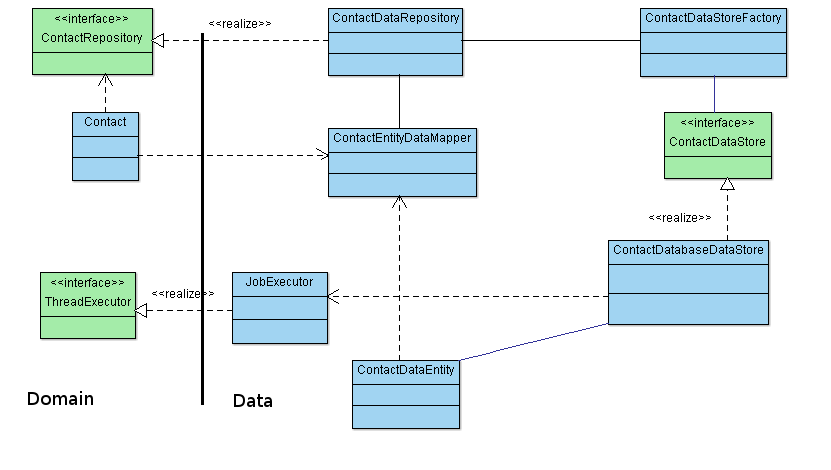
\includegraphics[width=0.8\linewidth]{../images/DataClasesDiagram}
		\caption{Diagrama de clases de la capa de datos}
		\label{fig:Clases de la capa Data}
	\end{figure}
	
	\subsection{Capa de Dominio}
	
	La capa de dominio esta basada en los casos de uso de la aplicación. Estos son interfaces que heredan de Interactor, que implementa Runable. De esta manera las implementaciones de los mismos contienen un ThreadExecutor implementado por JobExecutor en la capa de datos, al que se envian a sí mismos para ejecutar la acción del caso de uso. Por el otro lado, son los diferentes presenters de la aplicación, quienes implementan los diferentes casos de uso. 
	
		\begin{figure}[H]
			\centering
			\includegraphics[width=0.8\linewidth]{../images/DomainClasesDiagram}
			\caption{Diagrama de clases de la capa de dominio}
			\label{fig:Clases de la capa Domain}
		\end{figure}
	
	\subsection{Capa de Presentación}
	
	Esta capa se relaciona con el dominio mediante los presenters, que contienen las operaciones de los diferentes casos de uso que se relacionan en su vista. Ademas contienen interfaces sobre las clases de vista para que estas soporten los metodos que los propios presenters necesitan.
	
		\begin{figure}[H]
			\centering
			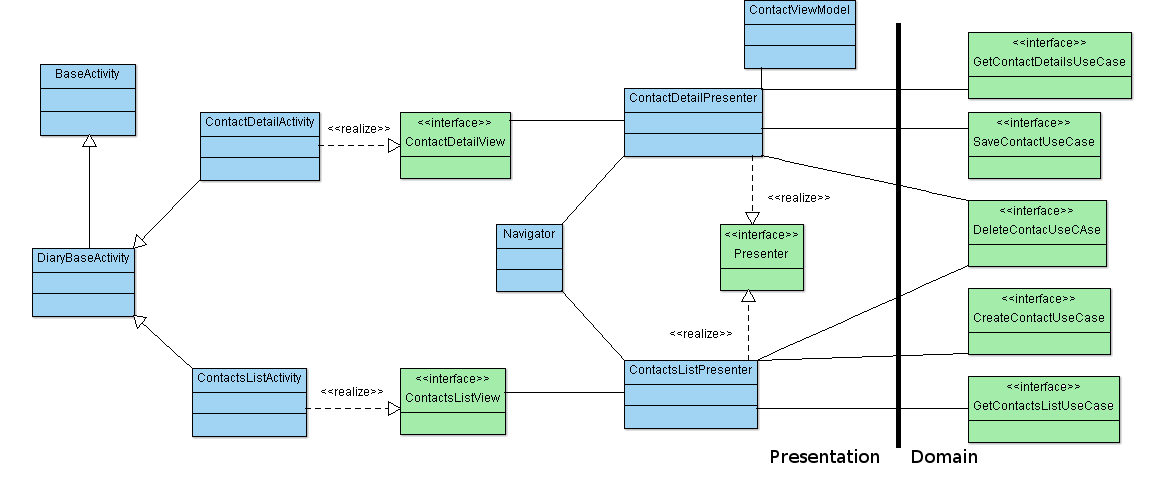
\includegraphics[width=0.8\linewidth]{../images/PresentationClasesDiagram}
			\caption{Diagrama de clases de la capa de presentación}
			\label{fig:Clases de la capa Presentation}
		\end{figure}
	
	\section{Diseño de la base de datos}

	
	\section{Prototipado}
	
	En la fase de diseño, el propósito del prototipo es obtener una primera versión de la apariencia de la interfaz de usuario así como de la funcionalidad incluida (mostrar las ventanas, su navegación, interacción, controles y botones). Con esto se pretende que el cliente tenga una primera toma de contacto con la futura aplicación antes de su desarrollo final, para así reducir o eliminar todas aquellas disconformidades y cambios en fases futuras.
	
		\subsection{Material Design}
		Material Design es la nueva metáfora visual de Matias Duarte para el sistema operativo móvil Android, en su version 5.0 y posteriores, y todo el ecosistema Google en web y supone una pequeña ruptura con la anterior metáfora de Android llamada Holo. \\*
		
		Es un diseño donde la profundidad, las superficies, los bordes, las sombras y los colores juegan un papel principal.
		
		Precisamente este diseño basado en objetos es una manera de intentar aproximarse a la realidad, algo que en un mundo donde todo es táctil y virtual es difícil. Material Design quiere guiarse por las leyes de la física, donde las animaciones sean lógicas, los objetos se superpongan pero no puedan atravesarse el uno al otro y demás.\\*
		
		Material Design es un diseño con una tipografía clara, casillas bien ordenadas, colores e imágenes llamativos para no perder el foco y un sentido del orden y la jerarquía muy marcado. Estas ideas ya se aplican en muchos diseños, pero en Material Design Google ha creado unas normas muy claras de como llevarlo a la práctica.\\*
		
		\subsection{Pantallas Principales}
		
		Pantallas iniciales y flujo de la aplicación que de manera inicial hemos planteado para la misma.
		No es la versión final de la aplicación pero si se aproxima y nos da una idea clara de lo que debería ser o a lo que debería parecerse.\\*
		
		Estos prototipos, sirven para orientarnos a la hora de construir la aplicación y sirven para que el cliente o product owner se haga una idea de hacia donde irá el desarrollo de la misma. Muchas de las pantallas proceden de una adaptación del libro que se utiliza en la AECC 'MIS CUIDADOS, diario de salud para supervivientes de cáncer'.\\*
		
		\begin{figure}[H]
			\centering
			
\includegraphics[width=0.4\linewidth]{../folleto/001_corto}
			\caption{Iniciativa de la AECC}
			\label{fig:001corto}
		\end{figure}
		
		Otras de las pantallas y funcionalidades, se han adaptado para facilitar el uso, adaptarse a los requerimientos del cliente y ampliar el rango de acción de este libro y hacerlo más lógico a nuestro entender.\\*
		
		
		
		\textbf{Pantalla Principal y Drawer menú}
		
		El usuario, al ejecutar la aplicación accede a una pantalla cuyo contenido es el listado de las actividades próximas a realizar, ya sea una cita médica o una rutina. En ausencia de las mismas, nos mostrará un mensaje alentándonos a realizar alguna rutina.\\*
		
		El drawer nos permite navegar entre actividades, desde la pantalla principal podemos añadir citas y acceder de manera individual a las mismas.\\*
	 
		
		\begin{figure}[H]
			\centering
			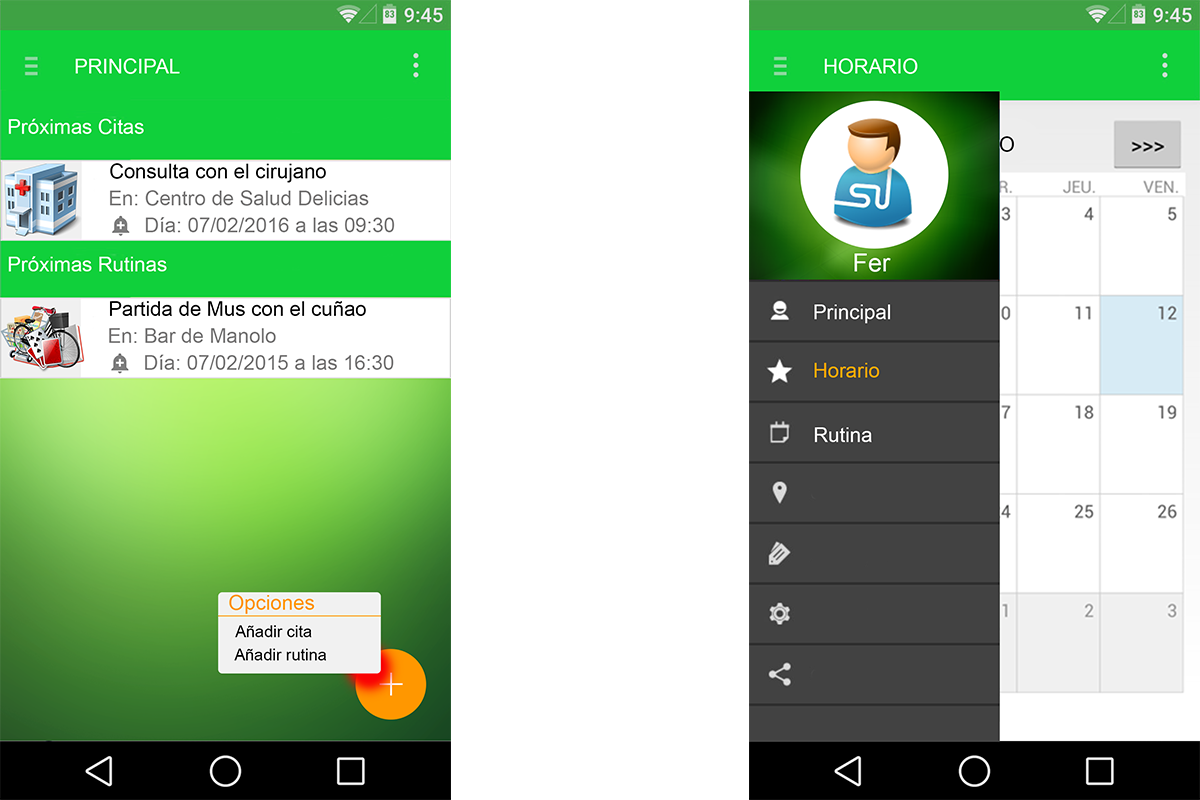
\includegraphics[width=0.8\linewidth]{../images/principal_2}
			\caption[Drawer menú y Pantalla principal]{Descripción de la pantalla principal y Drawer menú}
			\label{fig:principal}
		\end{figure}
		
		
		\textbf{Pantallas referentes a la programación de actividades}
		
		En la iniciativa de la asociación, se proporciona un cuadro para poder controlar las actividades que realizamos de manera rutinaria a lo largo de los días de la semana, ampliamos esta funcionalidad para que las citas se representen también el el horario.\\*
		
			\begin{figure}[H]
				\centering
				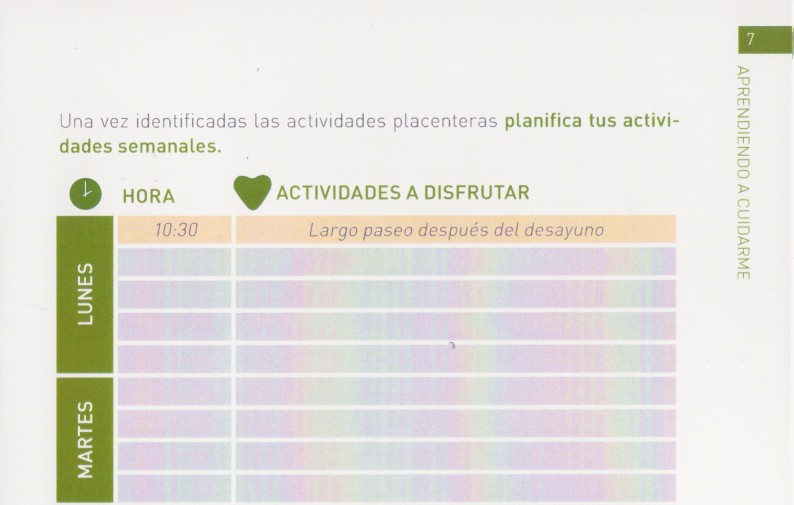
\includegraphics[width=0.7\linewidth]{../folleto/007_corto}
				\caption{Vista de los días en el folleto}
				\label{fig:horario_corto}
			\end{figure}
		
		
		Desde estás pantallas tenemos una visión de la ocupación diaria del paciente y de la ocupación mensual, desde la vista mensual al menos se podrán añadir nuevas citas médicas o rutinas para ese paciente.\\*

		
		\begin{figure}[H]
			\centering
			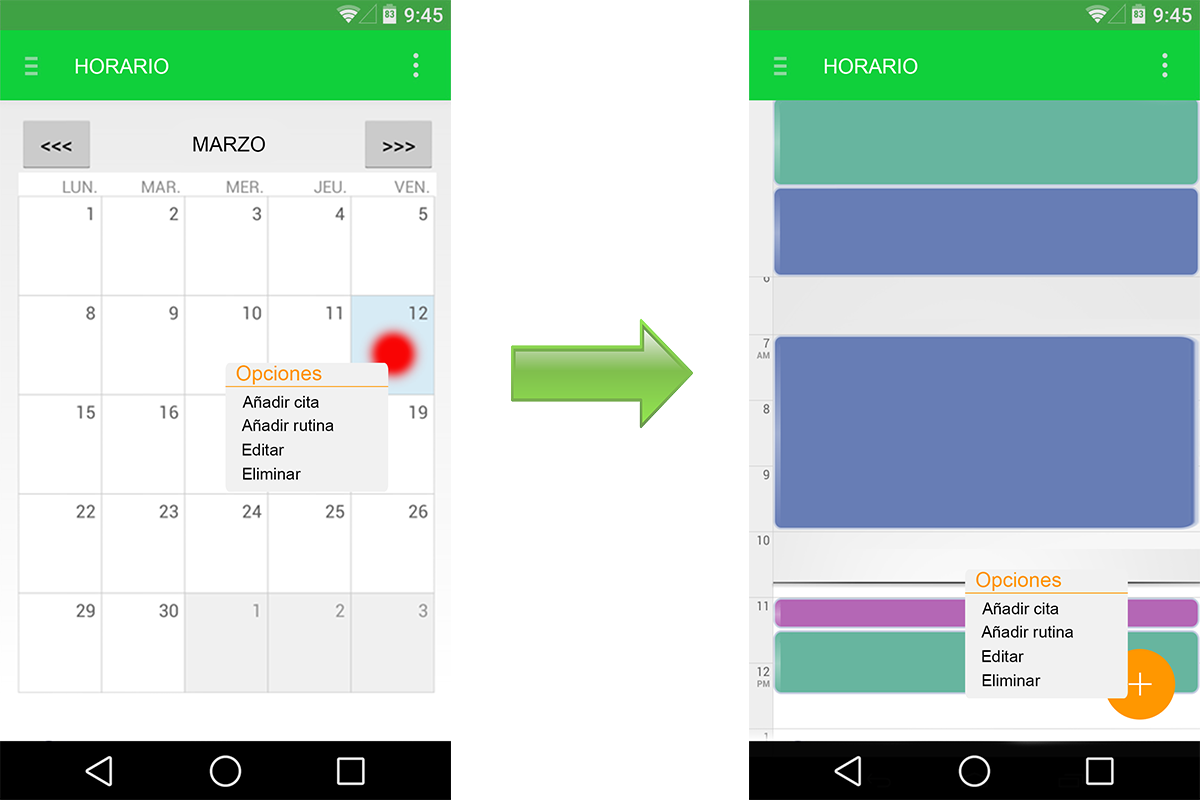
\includegraphics[width=0.7\linewidth]{../images/horario_2}
			\caption[Horario de actividades]{Pantallas con los horarios y ocupación del paciente}
			\label{fig:horario_2}
		\end{figure}
		
		
		\textbf{Pantallas referentes a la rutina diaria}
		
		Estas funcionalidades descienden directamente del libro proporcionado por la AECC, en el que como usuario integrado en el programa de mejora de la calidad de vida del superviviente de cáncer se le insta a realizar actividades que le produzcan cierta satisfacción y a realizarlas con asiduidad, sea en compañía o solo. En resumen se recomienda hacer actividades que nos hagan felices y nos animan a puntuarlas con el grado de satisfacción que nos producen las mismas. En el estracto del libro podemos apuntar la actividad, la fecha en la que la vamos a realizar, indicar quien nos acompaña, grado de satisfacción que nos produce y repetir.
		
		
		
		\begin{figure}[H]
			\centering
			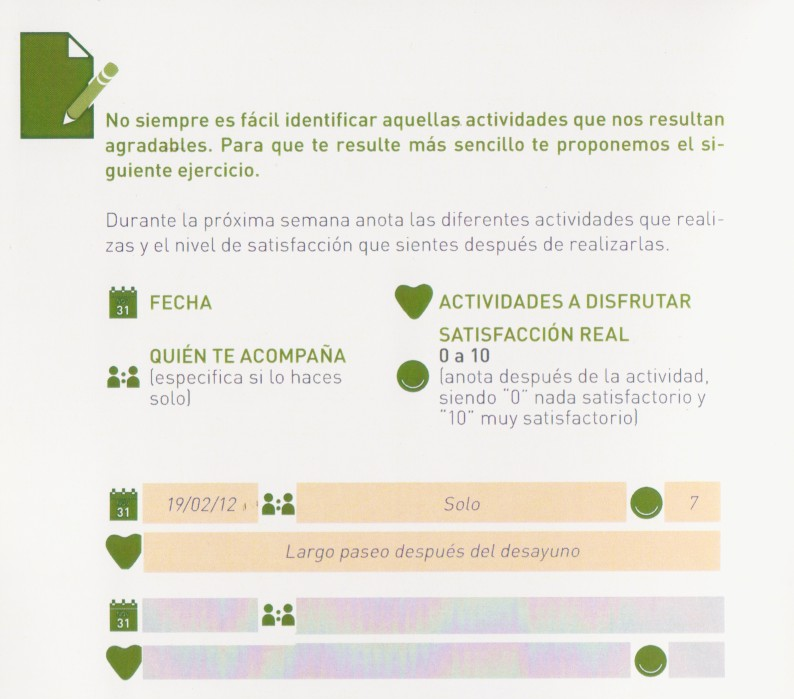
\includegraphics[width=0.7\linewidth]{../folleto/006_corto}
			\caption{Cuadro de actividades a realizar}
			\label{fig:006}
		\end{figure}

		
		Para la adaptación y mejora de las especificaciones del libro utilizado en la iniciativa, se ha diseñado un listado de las rutinas diarias que tiene ese paciente y representación de la introducción de una nueva rutina para ese paciente.\\*
		Dentro de la introducción de la rutina se podrán añadir nuevos personajes que acompañarán a ese paciente y le harán más fácil recordar con quien quedó y para qué.\\*

		
		\begin{figure}[H]
			\centering
			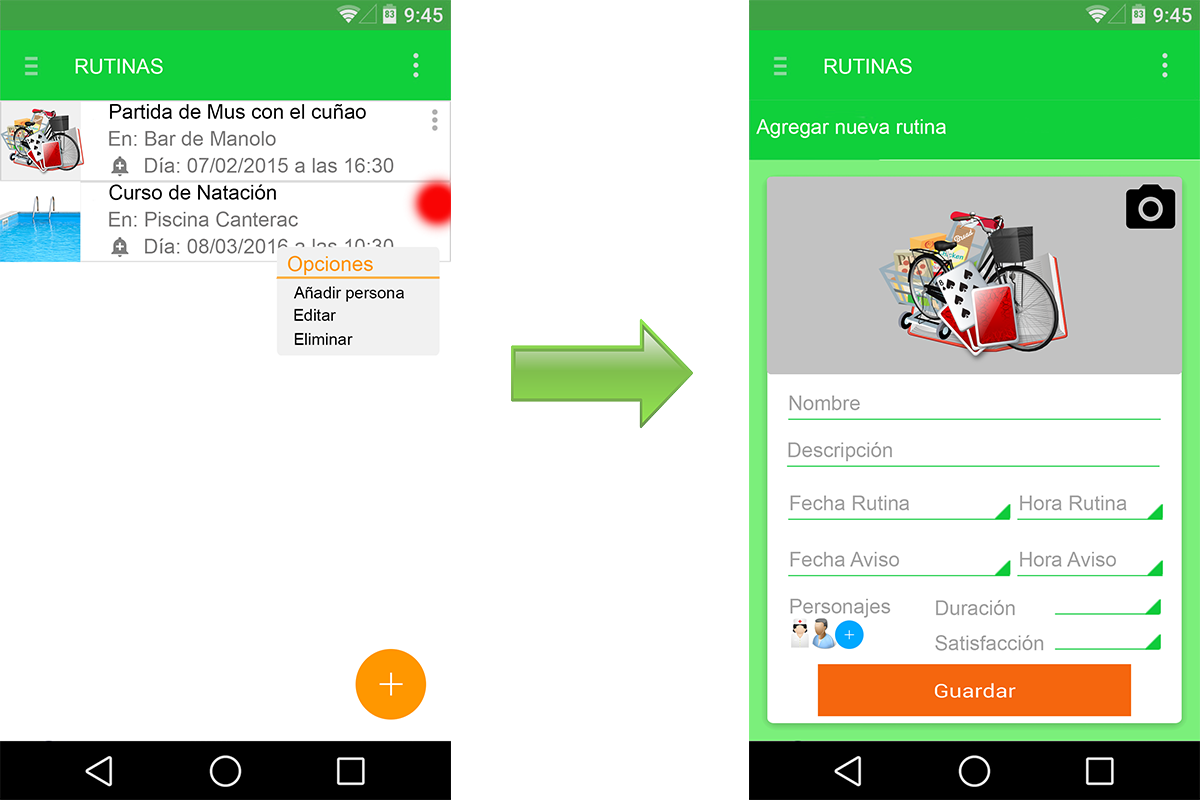
\includegraphics[width=0.7\linewidth]{../images/rutina}
			\caption{Pantalla con la interfaz para las rutinas}
			\label{fig:rutina}
		\end{figure}
					
		
		\textbf{Pantallas referentes a las citas médicas}
		
		Las páginas referentes a las citas médicas se basan en una serie de recomendaciones sobre como afrontar la visita al hospital, centro de salud, oncólogo y demás especialistas. Nos aporta una lista de cosas que deberíamos preguntar al especialista para rebajar la ansiedad ante la misma y sacar el máximo partido a la misma.\\*
		
		\begin{figure}[H]
			\centering
			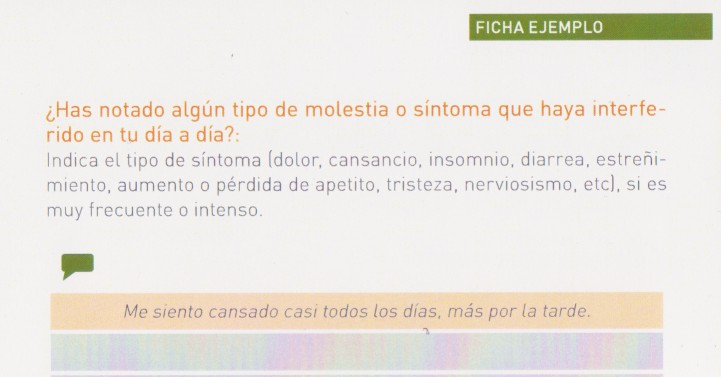
\includegraphics[width=0.7\linewidth]{../folleto/015_corto_a}
			\caption{Página con información a completar en la cita médica}
			\label{fig:preguntas}
		\end{figure}
		
		
		Listado de las citas medicas de ese paciente e introducción de la cita en si de manera individual.\\*
		De funcionamiento similar a las pantallas anteriores pero con diferencias sustanciales en la funcionalidad de la introducción de información, se pueden añadir personajes, síntomas, medicamentos y pruebas, de manera que el paciente cuando acuda a la cita lleve de manera ordenada toda esta información.\\*
		
		\begin{figure}[H]
			\centering
			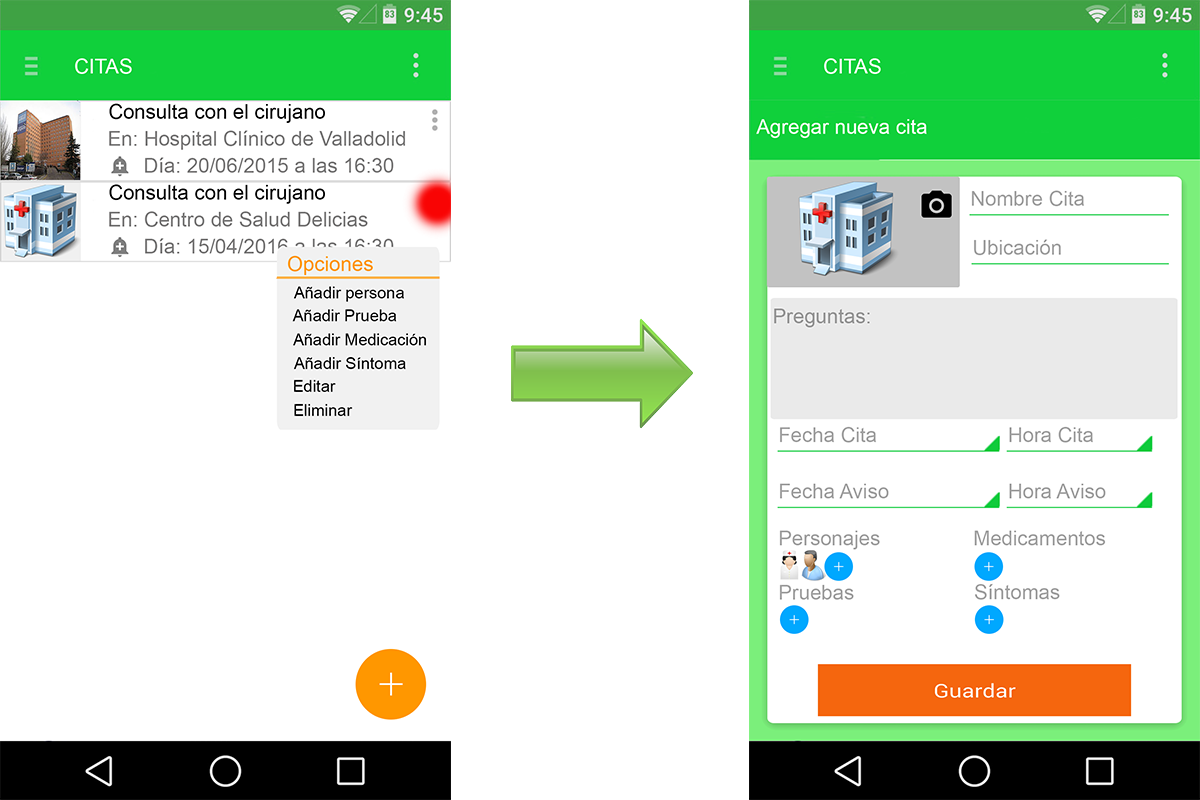
\includegraphics[width=0.7\linewidth]{../images/citas}
			\caption{Pantalla con la actividad de las citas}
			\label{fig:citas}
		\end{figure}
		
		
		\textbf{Pantallas referentes a la medicación}
		
		El libro nos proporciona un cuadro para el control de los medicamentos, nos permite apuntar el nombre sus indicaciones y parte de la posología del mismo, pero a nuestro modo de ver es algo insuficiente y se puede completar con notificaciones y más información que le permita ser identificado facilmente.
		
		\begin{figure}[H]
			\centering
			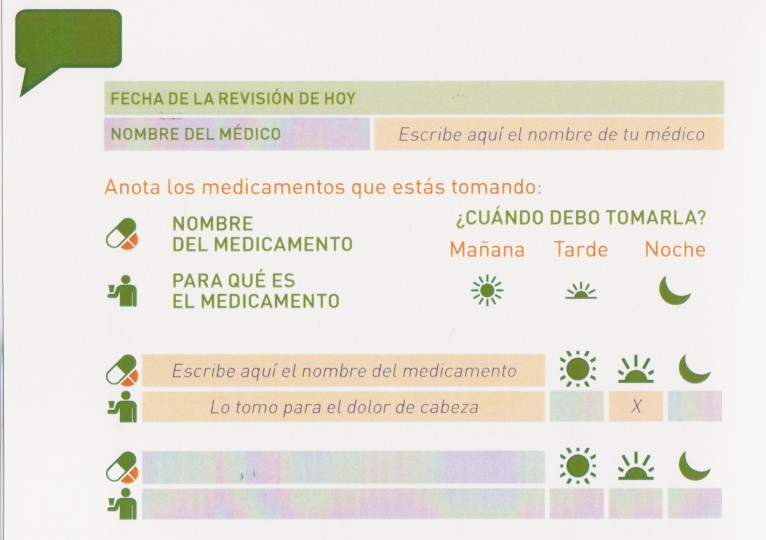
\includegraphics[width=0.7\linewidth]{../folleto/014_corto}
			\caption{Medicación y posología de los medicamentos}
			\label{fig:medicamentacion_libro}
		\end{figure}
				
		
		El usuario introduce los medicamentos que toma, de manera que puede añadir alertas a los mismos para que se le avise de que ha llegad la hora de la dosis con una notificación.
		Se podrán introducir otros datos del medicamento como pueden ser los intervalos entre dosis, indicaciones...\\*
		
		\begin{figure}[H]
			\centering
			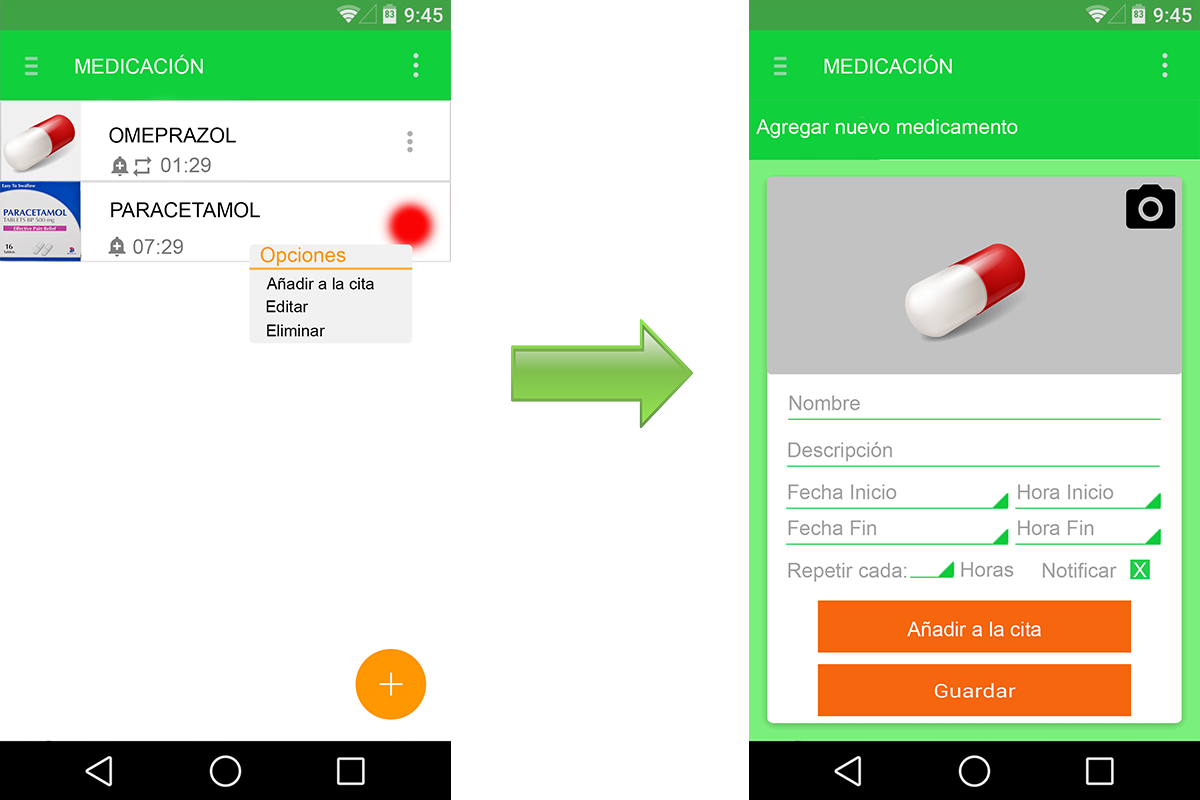
\includegraphics[width=0.7\linewidth]{../images/medicacion}
			\caption{Pantalla con la actividad de la medicación}
			\label{fig:medicacion}
		\end{figure}
		
		
		\textbf{Pantallas de gestión de personajes}
		El usuario puede añadir a la aplicación su lista de amigos, personal médico que le atiende, asistentes, etc, con sus datos personales, de manera que a la hora de hacer una rutina (actividad) o acudir a una cita, puedan ser añadidos.\\*
		
		
		\begin{figure}[H]
			\centering
			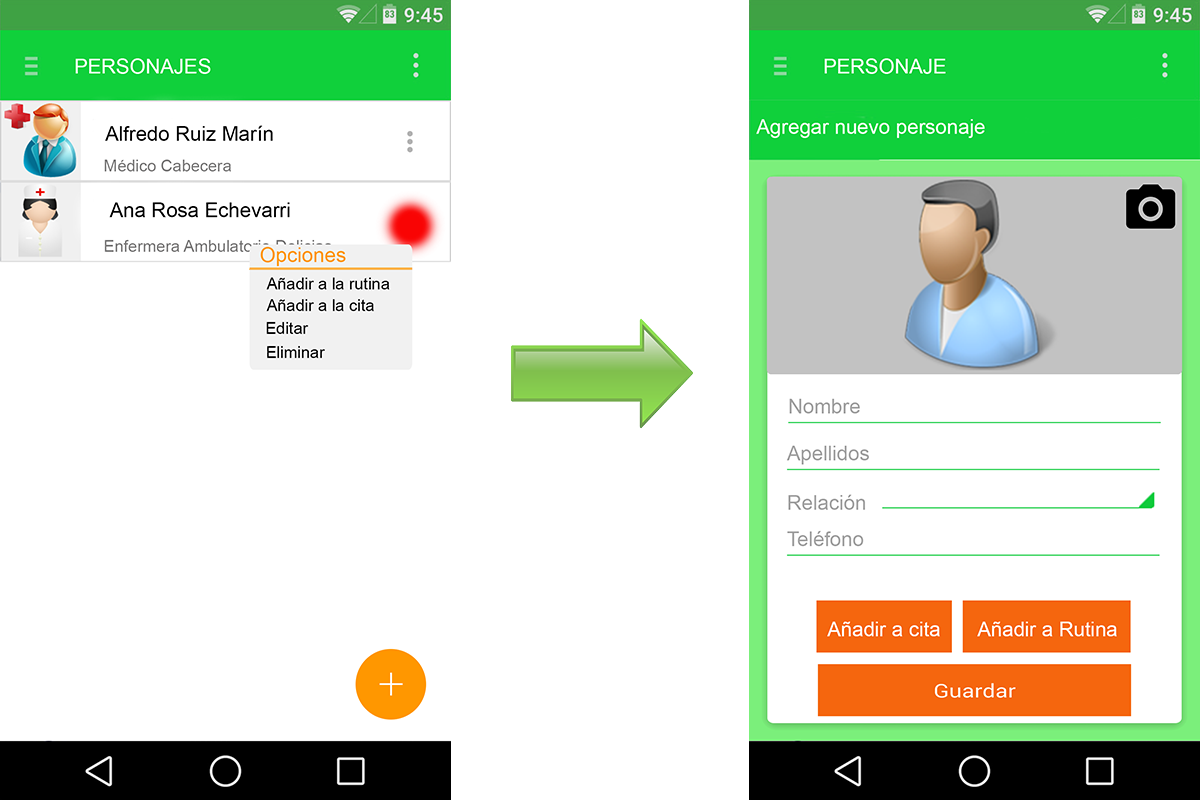
\includegraphics[width=0.7\linewidth]{../images/personajes}
			\caption{Pantalla con la actividad de los personajes}
			\label{fig:personajes}
		\end{figure}
		
		
		\textbf{Pantallas de gestión de pruebas médicas}
		Se facilita el poder llevar las pruebas médicas en forma de archivo fotográfico para poder consultarse en alguna de las citas medicas a las que acuda, tales como revisiones, visitas al fisio, a la enfermera. Listado del mismo.\\*
		
		\begin{figure}[H]
			\centering
			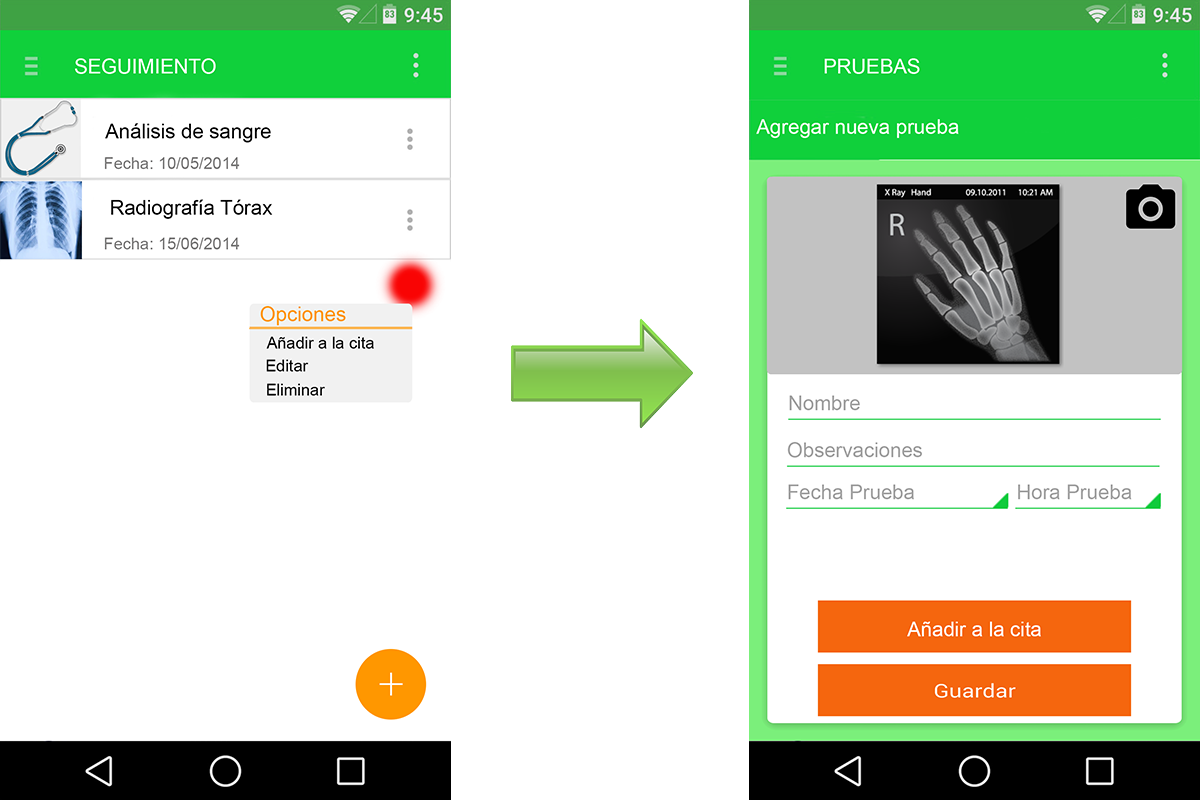
\includegraphics[width=0.7\linewidth]{../images/pruebas}
			\caption{Pantalla con la actividad de las pruebas}
			\label{fig:pruebas}
		\end{figure}
		
		
		\textbf{Pantallas de gestión de los síntomas}
		
		Los síntomas se apuntan en la misma ficha que los datos de la cita médica, con lo cual sería interesante que toda esa información se viese representada en la aplicacíon, hay que tenerla en cuenta en el flujo.
		
		\begin{figure}[H]
			\centering
			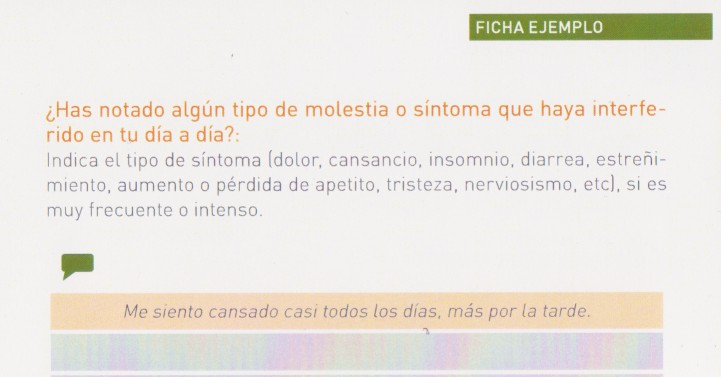
\includegraphics[width=0.7\linewidth]{../folleto/015_corto_a}
			\caption{Cuadro de los síntomas en el libro}
			\label{fig:sintomas_libro}
		\end{figure}
				
				

		El usuario puede tomar nota de los síntomas, molestias, efectos secundarios negativos o positivos que le acontecen, para poder asignarles después a una cita médica y poder completar de manera más eficiente las mismas, pudiendo aportar información adicional que ayude a su médico a mejorar el diagnóstico.\\*
		
		\begin{figure}[H]
			\centering
			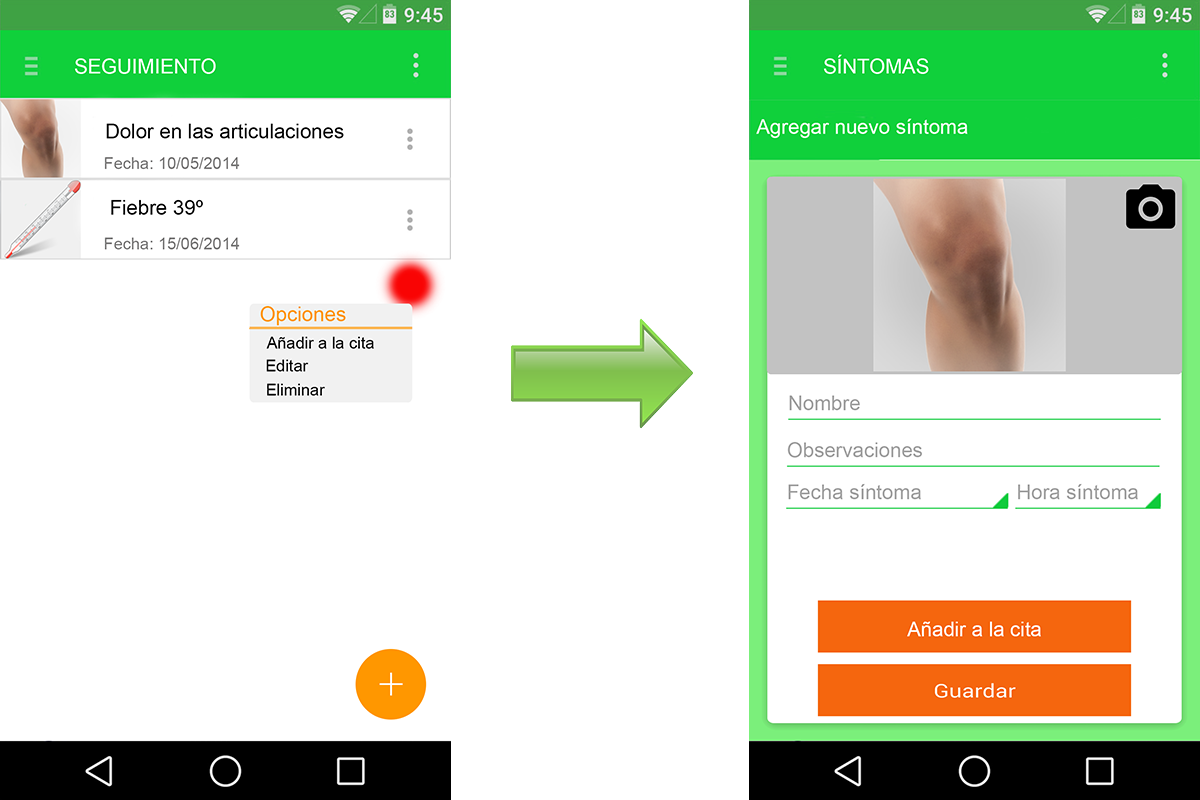
\includegraphics[width=0.7\linewidth]{../images/sintomas}
			\caption{Pantalla con la actividad de los síntomas}
			\label{fig:sintomas}
		\end{figure}
		
		
		\textbf{Pantallas de Recursos}
		
		A parte de todos los consejos que se dan el el libro sobre como afrontar la fase posterior a la enfermedad, se hace especial hincapié en la meditación, necesaria para proporcionar un estado relajado al superviviente, ante citas medicas importantes y que le generen tensión.\\*
		
		\begin{figure}[H]
			\centering
			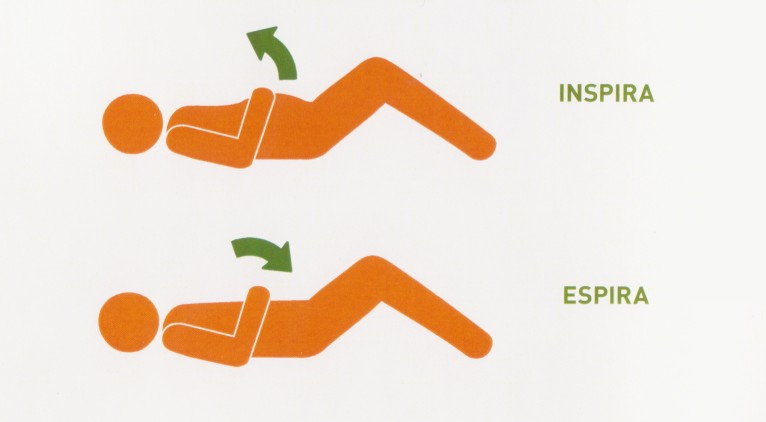
\includegraphics[width=0.7\linewidth]{../folleto/008_corto}
			\caption{Ejercicios de meditación}
			\label{fig:meditacion}
		\end{figure}
		
		Otra parte importante del libro es un listín telefónico en el que se pueden apuntar los contactos importantes, dirección, y números de teléfono. Toda esta parte se contempla en nuestra aplicación a través de los personajes y de los teléfonos de interés de la sección de recursos. 
		
		\begin{figure}[H]
			\centering
			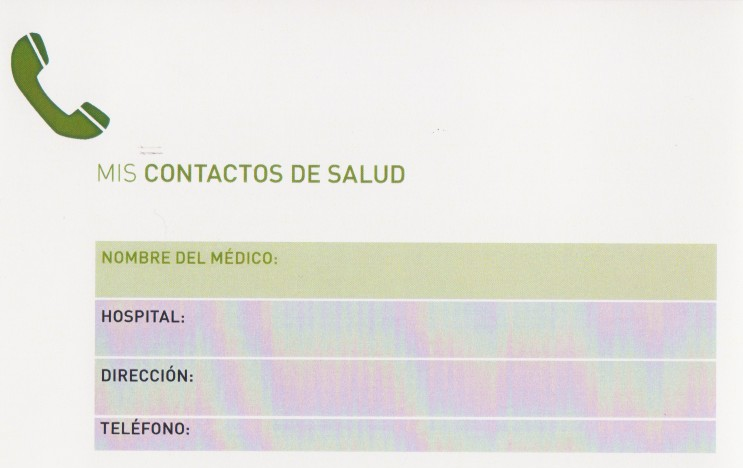
\includegraphics[width=0.5\linewidth]{../folleto/016_corto}
			\caption{Contactos importantes a tener en cuenta}
			\label{fig:contactos}
		\end{figure}
		
		
		
		Estas pantallas están pensadas para que el paciente disponga de ayuda adicional, y una serie de recursos de fácil acceso así como una sección de noticias de la AECC para que puedan ser consultadas por el paciente.
		Sección de meditación, consejos generales que le puedan ser de ayuda, noticias y teléfonos de interés. \\*
		
		\begin{figure}[H]
			\centering
			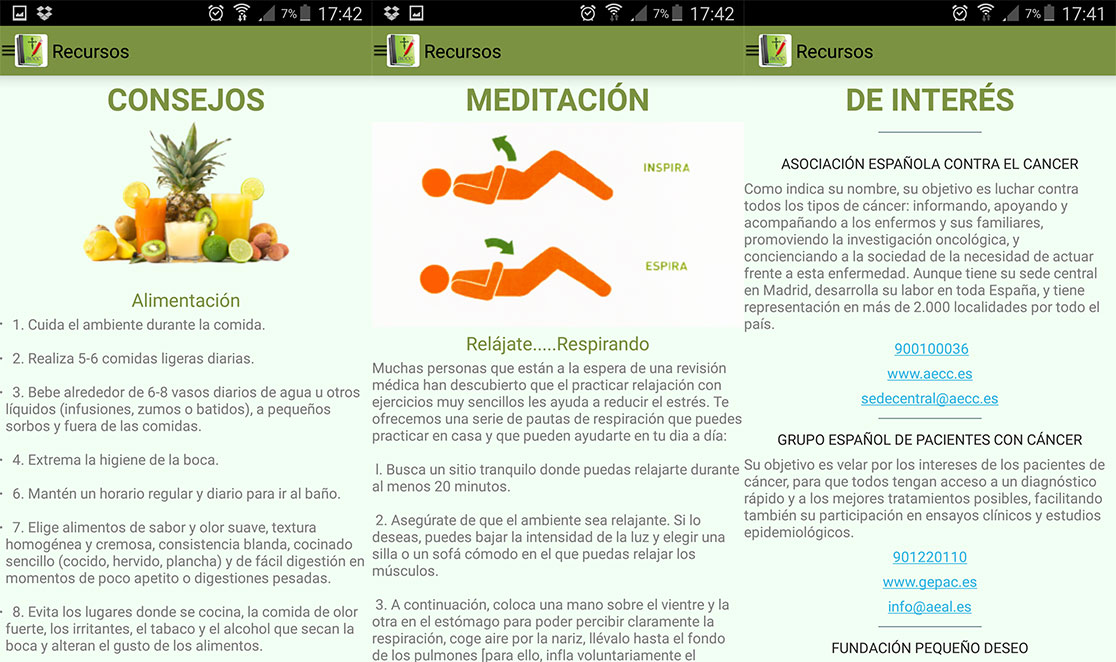
\includegraphics[width=0.9\linewidth]{../images/recursos}
			\caption{Pantalla con la actividad de los recursos}
			\label{fig:recursos}
		\end{figure}
		
		
		\textbf{Pantalla de perfil de usuario}
		El usuario podrá introducir sus datos personales para que la aplicación pueda tratarle de manera personalizada.\\*
		
		\begin{figure}[H]
			\centering
			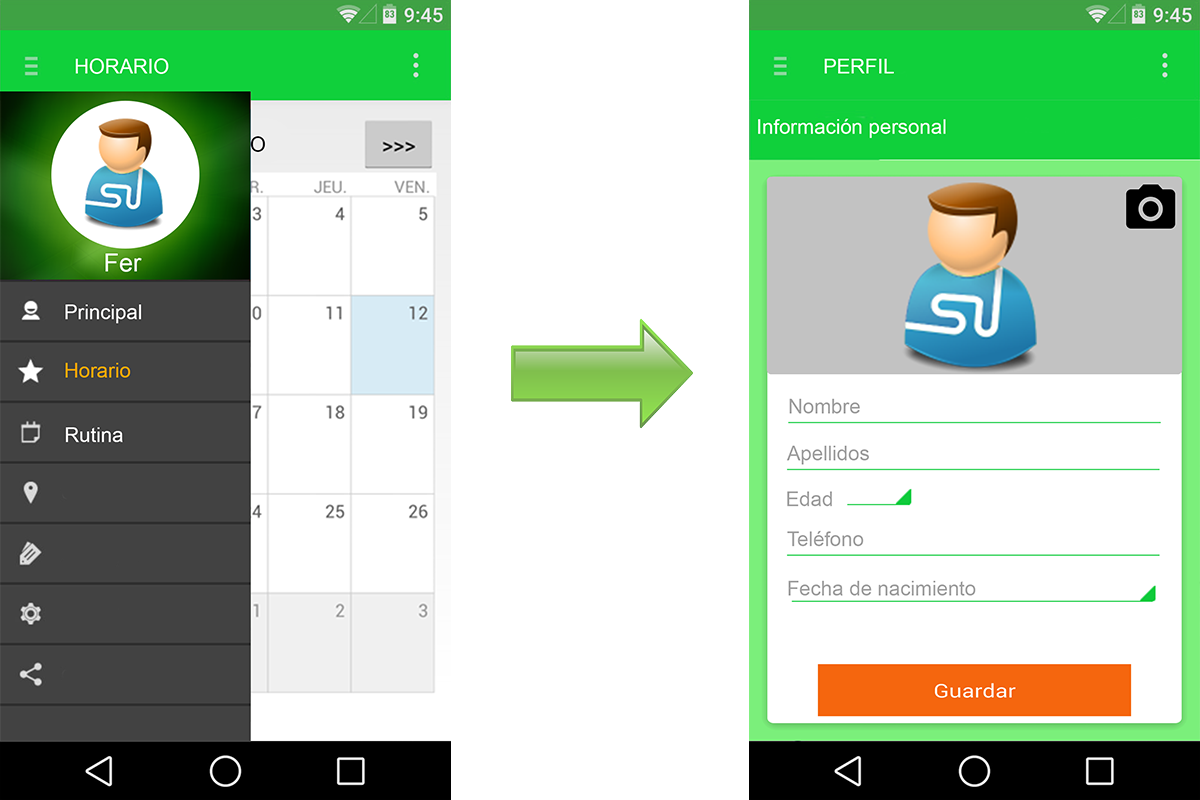
\includegraphics[width=0.7\linewidth]{../images/perfil_2}
			\caption{Pantalla con la actividad configuración del perfil}
			\label{fig:perfil_2}
		\end{figure}
		
		
		\textbf{Otros: Pantalla de presentación y carga}
		Pantalla inicial de carga, se utiliza para aportar más identidad a la aplicación y a modo de pequeña intro.\\*
		
		\begin{figure}[H]
			\centering
			
\includegraphics[width=0.3\linewidth]{../images/flasher_pantalla_carga}
			\caption{Pantalla de presentación de la aplicación}
			\label{fig:flasher_pantalla_carga}
		\end{figure}
		
	\clearpage		
	
	\section{Iconografía y otros cambios}
	
	A petición del Product Owner y dado que estamos trabajando con una metodología agil, los cambios y las adaptaciones en el diseño no son una excepción, los prototipos han ido variando en el tiempo con los cambios propuestos por el cliente y se ha adaptado para proporcionar una imagen más 'corporativa' y en consonancia con la iniciativa en la que está situado.
	
		\begin{figure}[H]
			\centering
			
\includegraphics[width=0.5\linewidth]{../images/icon_aecc}
			\caption{Icono de la aplicación principal}
			\label{fig:icono}
		\end{figure}
	
	
	La imagen visible de la aplicación, incluso antes de acceder a la misma, va a ser su icono, este nos tiene que dejar entrever parte de la intención de la aplicación y ser fácilmente identificable entre el resto de los iconos de las aplicaciones instaladas.
	
			\begin{figure}[H]
				\centering
				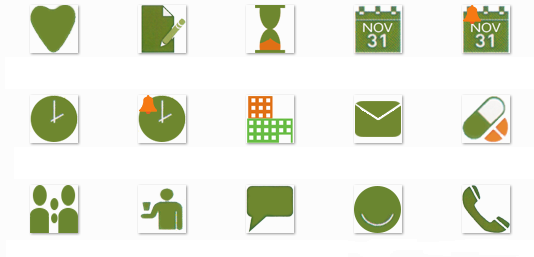
\includegraphics[width=0.7\linewidth]{../images/iconografia}
				\caption{Conjunto de iconos de apoyo para las pantallas de las entidades}
				\label{fig:iconografia}
			\end{figure}	
	
	
	Se diseñaron gran parte de los iconos que forman parte de las pantallas, con un aspecto que recuerda al del libro y con un estilo acorde al que se utiliza en el mismo folleto, para que el usuario tengo una experiencia de uso que le muestre continuidad.
	
	También se re-diseñaron algunas de las pantallas principales para hacerlas más fácilmente identificables con el libro de la iniciativa de la asociación y mantener la coherencia visual del proyecto.
	
	  
			\begin{figure}[H]
				\centering
				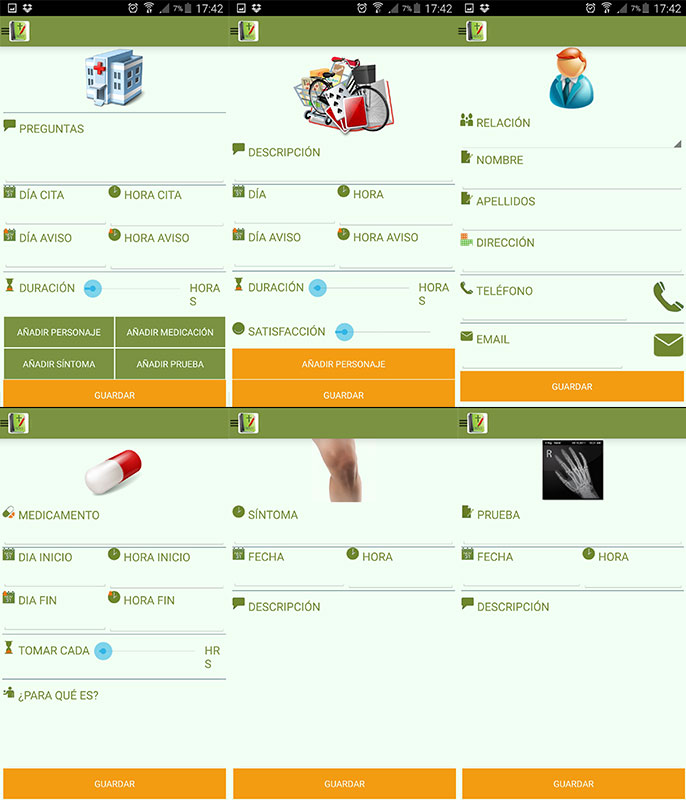
\includegraphics[width=1\linewidth]{../images/new_prot}
				\caption{Nuevo diseño de las pantallas generales de la aplicación}
				\label{fig:rediseno}
			\end{figure}
			
	\clearpage			
	
	Por último, la parte de recursos sufrió algunas modificaciones, la parte en la que se insertarían noticias de la AECC se ha suprimido para no perder el foco de la verdadera utilidad de la aplicación y dado que la asociación dispone de otros canales para la propagación de las mismas, se consideró oportuno su supresión en esta versión.\\*
	
	Con lo cual, recursos ha quedado de la siguiente manera, una pestaña de consejos generales, una pestaña de meditación y relajación y una pestaña de asociaciones y páginas de interés.
	
	\begin{figure}[H]
		\centering
		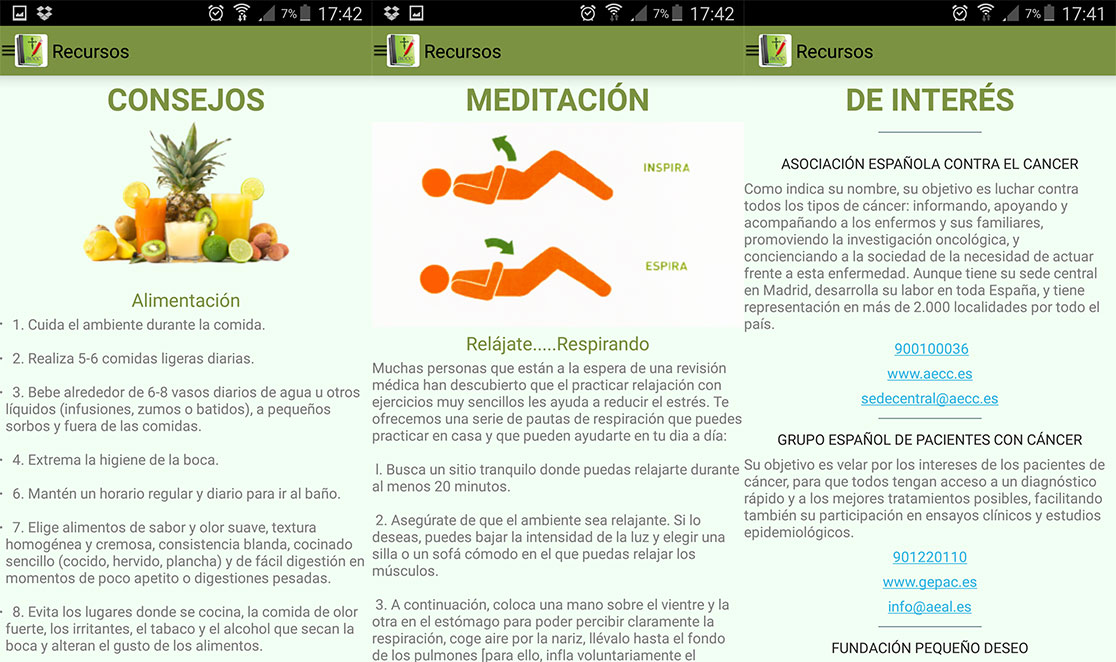
\includegraphics[width=1\linewidth]{../images/recursos_B}
		\caption{Nuevo diseño de los recursos}
		\label{fig:redisenoRecursos}
	\end{figure}
	

	
	
	
\end{document}